\documentclass{beamer}
\usepackage[utf8]{inputenc}
\usepackage{amsmath,amsfonts,amsthm,amstext,amssymb, xcolor, tikz, pgf}

% ----------------------------------------------------------
% Theme Setup

% Use Metropolis Theme
\usetheme[numbering=fraction]{metropolis}
\setbeamertemplate{blocks}[rounded][shadow=false]
\makeatletter
\setlength{\metropolis@titleseparator@linewidth}{1pt}
\makeatother

% Define Colors
\definecolor{chargerblue}{HTML}{002764}
\definecolor{chargerred}{HTML}{e02034}
\definecolor{bggray}{HTML}{d0d3d4}

% Set Colors
\setbeamercolor{title}{fg=chargerblue}
\setbeamercolor{background canvas}{bg=white}
\setbeamercolor{title separator}{fg=chargerred}
\setbeamercolor{structure}{fg=chargerblue}
\setbeamercolor{frametitle}{fg=white, bg=chargerblue}
\setbeamercolor*{normal text}{fg=chargerblue}
\setbeamercolor*{block body}{bg=bggray}
\setbeamercolor*{block title}{bg=chargerblue, fg=white}
% ----------------------------------------------------------

% ----------------------------------------------------------
% Custom Definitions, Commands, Environments, etc.

% Sets of numbers
\def\R{\mathbb{R}} % The reals
\def\N{\mathbb{N}} % The naturals
\def\Z{\mathbb{Z}} % The integers
\def\Q{\mathbb{Q}} % The rationals

% Blank space
\newcommand{\blank}[1]{\underline{\hspace{#1}}} % Blank space

% Fitted inclusion symbols
\newcommand{\fp}[1]{\left({#1}\right)} % Fitted parentheses around content
\newcommand{\fb}[1]{\left[{#1}\right]} % Fitted brackets
\newcommand{\set}[1]{\left\{{#1}\right\}} % Fitted braces (useful for sets)
\newcommand{\av}[1]{\left|{#1}\right|} % Fitted absolute value bars



% Coordinate Plane (Four-Quadrant)
\def\coordplane {
	\begin{tikzpicture}		\draw[step=0.25cm,black,very thin,opacity=0.25] (-2.5cm, -2.5cm) grid (2.5cm, 2.5cm);
		\draw[<->,thick,black] (-2.5cm, 0) -- (2.5cm, 0) node[anchor=north west,pos=0.94,font=\scriptsize]{$x$};
		\draw[<->,thick,black] (0,-2.5cm) -- (0, 2.5cm) node[anchor=south east,font=\scriptsize,pos=0.94]{$y$};
	\end{tikzpicture}
}

% Coordinate Plane (One-Quadrant)
\def\onequad {
	\begin{tikzpicture}
		\draw[step=0.25cm, black, very thin, opacity=0.25] (0,0) grid (7.5cm,5cm);
		\draw[->, thick, black] (0,0) -- (7.5cm, 0) node[anchor=north west,font=\scriptsize,pos=0.94]{$x$};
		\draw[->, black, thick] (0,0) -- (0,5cm) node[anchor=south east,font=\scriptsize,pos=0.94]{$y$};
	\end{tikzpicture}
}
% ----------------------------------------------------------

% ----------------------------------------------------------
% Presentation Information 
\title[2.1 and 2.2]{Linear Equations in Two Variables; Functions}
\subtitle{Sections 2.1 and 2.2}
\author{Jacob Ayers}
\institute{Lesson \#8}
\date{MAT 130}
% ----------------------------------------------------------

\begin{document}

% Slide 1 (Title Slide)
\begin{frame}
\titlepage
\end{frame}

% Slide 2 (Objectives)
\begin{frame}[t]{Objectives}
\begin{itemize}
	\item Compute slopes of lines
	\item Graph linear equations written in slope-intercept and point-slope forms
	\item Use slope to determine when lines are parallel or perpendicular
	\item Solve applied problems involving slope
	\item Determine whether a relation represents a function
	\item Evaluate functions, including piecewise functions
	\item Find the domain of a function
	\item Solve applied problems involving functions
\end{itemize}
\end{frame}

\begin{frame}[t]{Key Definitions Relating to Lines}
\begin{block}{Definition}
A \textit{linear equation in two variables} is an equation that can be written in the form $$y = mx + b$$
\end{block}

\pause

\begin{block}{Definition}
The \textit{slope} of a nonvertical line (usually denoted by $m$) is the number of units the line rises (or falls) vertically for each unit of horizontal change from left to right.
\end{block}

\pause

\begin{block}{Definition}
The \textit{slope-intercept form of a linear equation} is $$y = mx + b$$
The slope of the line is $m$ and the $y$-intercept is $(0, b)$.
\end{block}
\end{frame}

\begin{frame}[t]{Sketching Graphs of Lines}
Sketch the graph of the equation $y=3x+2$.

\coordplane
\end{frame}

\begin{frame}[t]{Sketching Graphs of Lines}
Sketch the graph of the equation $4x + y = 5$.

\coordplane
\end{frame}

\begin{frame}[t]{Finding Slope of a Line}
To find the slope of a line given its graph, you can use the formula $$m = \dfrac{\text{rise}}{\text{run}}$$ The rise is the vertical change and the run is the horizontal change. \vspace{18pt}

\pause To find the slope between two points $(x_1, y_1)$ and $(x_2, y_2)$, you can use the formula
$$m = \dfrac{y_2 - y_1}{x_2 - x_1}$$
\end{frame}

\begin{frame}[t]{Finding Slope of a Line}
Find the slope of the following line:

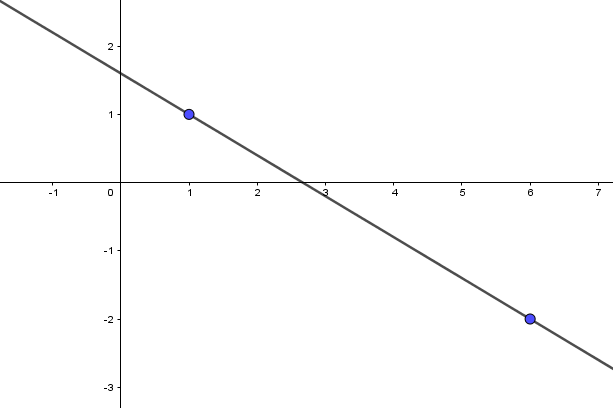
\includegraphics[width=3in]{SlopeLine1.png}
\end{frame}

\begin{frame}[t]{Finding Slope of a Line}
Find the slope between $(3, 8)$ and $(7, 14)$
\begin{flalign*}
\onslide<2->{m &= \dfrac{y_2 - y_1}{x_2 - x_1} & \\}
\onslide<3->{&= \dfrac{14 - 8}{7 - 3} & \\}
\onslide<4->{&= \dfrac{6}{4} = \dfrac{3}{2} &}
\end{flalign*}
\onslide<5->{Find the slope between $(2, 0)$ and $(2, 5)$}
\begin{flalign*}
\onslide<6->{m &= \dfrac{5 - 0}{2 - 2} & \\}
\onslide<7->{&= \dfrac{5}{0} & \\}
\onslide<8>{&\therefore \text{Slope is undefined}}
\end{flalign*}
\end{frame}

\begin{frame}[t]{Point-Slope Form}
\begin{block}{Definition}
The \textit{point-slope form of a line} is $$y - y_1 = m(x-x_1)$$ The line has a slope of $m$ and passes through the point $(x_1,y_1)$
\end{block}

\pause

Write an equation of a line passing through $(-2, 5)$ with a slope of $-\dfrac35$.

\pause $y - 5 = -\dfrac35(x + 2)$
\end{frame}

\begin{frame}[t]{Parallel and Perpendicular Lines}
\begin{block}{Parallel and Perpendicular Lines}
\begin{enumerate}[1)]
\item Two distinct lines are \textit{parallel} if their slopes are the same ($m_1 = m_2$)
\item Two nonvertical lines are \textit{perpendicular} if their slopes are opposite reciprocals $\fp{m_1 = -\dfrac{1}{m_2}}$
\end{enumerate}
\end{block}
\end{frame}

\begin{frame}[t]{Parallel and Perpendicular Lines}
Find the slope-intercept form of a line that passes through the point $(-4, 1)$ and is parallel to the line $5x - 3y = 8$.

\pause

First, we should write the given equation in slope-intercept form so we can easily find the slope:
\begin{flalign*}
5x - 3y &= 8 & \\
-3y &= -5x + 8 & \\
y &= \dfrac53 x - \dfrac83
\end{flalign*}
\pause
The slope of the original line is $\dfrac53$. \pause We are asked to find a parallel line, so its slope will also be $\dfrac53$.
\end{frame}

\begin{frame}[t]{Parallel and Perpendicular Lines}
Find the slope-intercept form of a line that passes through the point $(-4, 1)$ and is parallel to the line $5x - 3y = 8$.

We saw on the last slide that our line will have a slope of $\dfrac53$ and pass through $(-4,1)$. We can use this information to write a point-slope equation, then convert that to slope-intercept.
\begin{flalign*}
\onslide<2->{y - 1 &= \dfrac53(x + 4) & \\}
\onslide<3->{y - 1 &= \dfrac53 x + \dfrac{20}{3} & \\}
\onslide<4>{y &= \dfrac{5}{3}x + \dfrac{23}{3}}
\end{flalign*}
\end{frame}

\begin{frame}[t]{Parallel and Perpendicular Lines}
Find the slope-intercept form of a line that passes through the point $(3, 5)$ and is perpendicular to $y = 2x + 2$.

\pause This equation is already written in slope-intercept form; its slope is $2$. So the slope of the perpendicular line is $-\dfrac12$.
\pause
\begin{flalign*}
y - 5 &= -\dfrac12(x - 3) & \\
y - 5 &= -\dfrac12 x + \dfrac32 & \\
y &= -\dfrac12 x + \dfrac{13}{2}
\end{flalign*}
\end{frame}

\begin{frame}[t]{Slope in Applications}
In real-life problems, slope is either a ratio or a rate.
\pause

Example: The maximum recommended slope of a wheelchair ramp is $\dfrac{1}{12}$. A business installs a ramp that rises 36 inches over a length of 32 feet. Is the ramp steeper than recommended? \vspace{12pt}

\pause First, note that 36 inches is 3 feet. \pause So the slope of the ramp is $\dfrac{3}{32} = 0.09375$. \vspace{12pt}

\pause $\dfrac{1}{12} \approx 0.0833 < 0.09375$; our ramp is steeper than recommended.
\end{frame}

\begin{frame}[t]{Slope in Applications}
A manufacturing firm purchased a machine worth \$24750. The machine has a useful life of 6 years. After 6 years, it will need to be discarded and replaced because it will have no salvage value. Write a linear equation that describes the book value of the machine each year.

\pause

We will need to find the slope and the $y$-intercept.

\pause

The slope is $m = \dfrac{-24750}{6} = -4125$ dollars per year, and the $y$-intercept is $24750$ since that is the machine's value at time $0$.

\pause

So an equation that describes the machine's value is $y = -4125x + 24750$.
\end{frame}

\begin{frame}[t]{Functions}
\begin{block}{Definition}
A \textit{relation} is a rule that relates two quantities.
\end{block}

\begin{block}{Definition}
A \textit{function} $f$ from a set $A$ to a set $B$ is a relation that assigns each element $x \in A$ exactly one element $y \in B$. We call $A$ the \textit{domain} (inputs) and $B$ the \textit{range} (outputs).
\end{block}
\end{frame}

\begin{frame}[t]{Functions}
\begin{block}{Characteristics of Functions from $A$ to $B$}
\begin{enumerate}[1)]
\item Each element of $A$ is mapped to an element in $B$
\item Some elements in $B$ may not be matched with any element in $A$
\item Two or more elements of $A$ may be matched with the same element in $B$
\item No element in $A$ is mapped to more than one element in $B$
\end{enumerate}
\end{block}

Function Notation: $y = f(x)$ is read as ``$y$ is a function of $x$"; $y$ and $f(x)$ are interchangeable
\end{frame}

\begin{frame}[t]{Testing for Functions}
Determine whether each relation represents a function:

a) 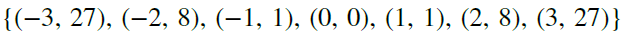
\includegraphics[scale=0.5]{Function1.png} \\
\pause This is a function. \vspace{12pt}

\pause b) \\
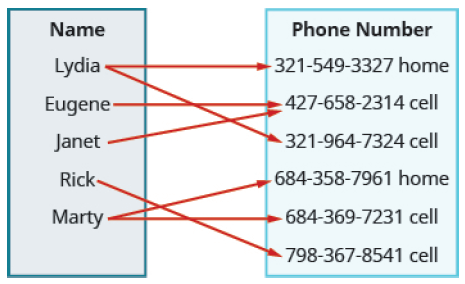
\includegraphics[scale=0.4]{Function2.png} \\
\pause This is not a function; Lydia maps to two different phone numbers.
\end{frame}

\begin{frame}[t]{Testing for Functions Represented Algebraically}
There are two methods of testing an equation to see if it represents a function: \begin{enumerate}[1)]
\item Graph it and use the Vertical Line Test
\begin{itemize}
\item If no vertical line touches the graph twice, it's a function; otherwise, it's not
\end{itemize}
\item Solve it for $y$ and see if it is possible for a single value of $x$ to map to two different values of $y$
\end{enumerate}
\end{frame}

\begin{frame}[t]{Testing for Functions Algebraically}
Does $x^2 + y^2 = 8$ represent a function?

\pause Graphically: \\
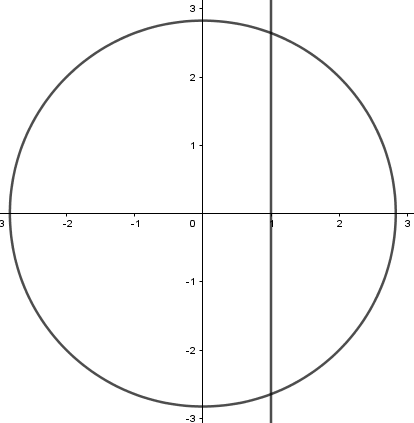
\includegraphics[scale=0.25]{CircleGraph.png} \\
\pause Fails the Vertical Line Test; not a function

\pause

Algebraically:
$y^2 = 9 - x^2 \Rightarrow y = \pm\sqrt{9 - x^2}$ \\
\pause The $\pm$ indicates that one $x$ can go to two different $y$'s; not a function
\end{frame}

\begin{frame}[t]{Evaluating Functions}
To evaluate a function $f(x)$ at a given value of $x$, plug the expression in parentheses into the equation that represents the function.

\pause Example: Evaluate $f(3)$ if $f(x) = 7 - 4x^2$

\pause $f(3) = 7 - 4(3)^2 = 7 - 36 = -29$ \vspace{8pt}

\pause

Example: Evaluate $V(3r)$ if $V(x) = 4\pi r^2$
\pause
\begin{flalign*}
V(3r) &= 4\pi (3r)^2 & \\
&= 4\pi(9r^2) & \\
&= 36\pi r^2
\end{flalign*}
\end{frame}

\begin{frame}[t]{Piecewise-Defined Functions}
\begin{block}{Definition}
A \textit{piecewise-defined function} is a function that is defined by two or more equations over a specified domain.
\end{block}

\pause Here is an example: $f(x) = \begin{cases} 2x + 3 & x \leq 2 \\ \sqrt{2x + 3} & x > 2 \end{cases}$ \vspace{12pt}

\pause To evaluate this function: if $x \leq 2$ then plug into the top equation. If $x > 2$ then plug into the bottom equation.

\pause Examples: \\ $f(0) = 2(0) + 3 = 3$ \\ $f(11) = \sqrt{2(11) + 3} = \sqrt{25} = 5$
\end{frame}

\begin{frame}[t]{An Application of Functions}
A second baseman throws a baseball toward the first basman 60 feet away. The path of the baseball is given by $$f(x) = -0.004x^2 + 0.3x + 6$$ where $f(x)$ is the height of the baseball in feet and $x$ is the horizontal distance from the second baseman in feet. The first baseman can reach 8 feet high. Can the first baseman catch the ball without jumping?

\pause

We'd like to know the height of the ball when it is 60 feet away from the second baseman; we need to find $f(60)$.

\pause

$f(60) = -0.004(60)^2 + 0.3(60) + 6 = 9.6$

\pause

The ball will be too high for the first baseman to reach without jumping.
\end{frame}

\begin{frame}[t]{Next Steps}
\begin{itemize}
\item Post questions in the Lesson 8 Forum, if you have them
\item Complete Assignment \#4
\item Begin Module \#5
\begin{itemize}
\item Read 2.3-2.5
\item Watch Video Lesson \#9
\end{itemize}
\end{itemize}
\end{frame}

\end{document}